\section{Using GraphRNN for Lattices Modeling\label{sec:graph-model}}

The architecture we propose to model lattices as graphs is an implementation of GraphRNN as a constrained VAE.
We first detail the workings of the original GraphRNN in \cref{sec:graph-model-graphrnn} and then present our adapted architecture in \cref{sec:graph-model-full}. 

\subsection{GraphRNN\label{sec:graph-model-graphrnn}}
This subsection is a quick overview of the inner workings of GraphRNN. For a detailed explanation, see~\cite{graphrnn:2018:jiaxuan}.

GraphRNN is a model for graph modeling composed of 2 components:
a \textit{graph-level} GRU to generate nodes, and a \textit{node-level} GRU to generate edges.
For each step of the graph-level model, the node-level model generates the edges with the previous nodes in the sequence.
In other words, the node-level model predicts the adjacency vector $S^\pi_i$ described in \cref{sec:level-order}.
The adjacency vector predicted by the node-level model is taken into account for the next step of the graph-level model.
The model can be considered in two phases: training and inference. They respectively correspond to training the model and using the model to generate new graphs.

In practice, the graph-level model generates a representation of a node's adjacency at each step, as a fixed-sized vector serving to initialize the node-level model.
This node representation is used as the first hidden state of the node-level RNN.
At each step, the node-level model predicts the probability of an edge existing between the currently processed node and one of the previous nodes.
During inference, this probability is used to randomly sample the edge, which is then used as the input of the next step of the node-level model.
During training the true previously edge is used instead.
\cref{fig:graphrnn} is an example of how the model unfolds when during inference.

The TensorFlow (an alternative to PyTorch) implementation of GraphRNN is available in the Snap Stanford repository\footnote{\url{https://github.com/snap-stanford/GraphRNN}}.

\begin{figure}
    \centering
    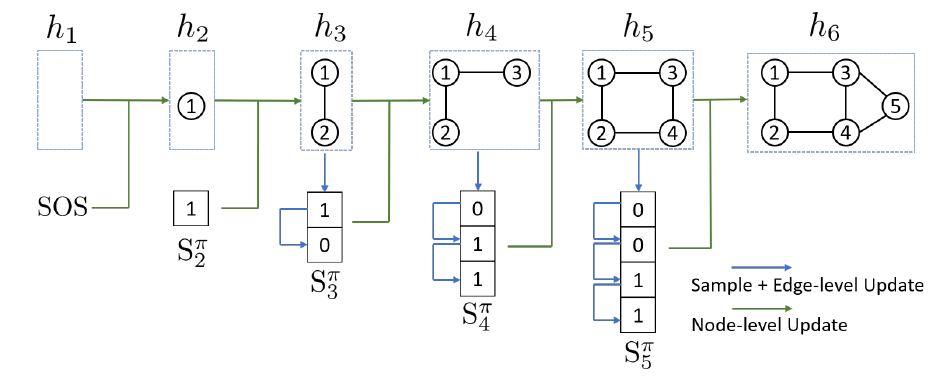
\includegraphics[keepaspectratio, width=.9\textwidth, height=4cm]{Figures/Ch1/graphrnn.png}
    \caption{GraphRNN at inference time. Figure 1 from~\cite{graphrnn:2018:jiaxuan}.}
    \label{fig:graphrnn}
\end{figure}

\subsection{GraphRNN Constrained VAE\label{sec:graph-model-full}}
%\todo[inline]{the planned setup, with intent/extent modeling}

To have a model able to generate lattices from FC based on the graph structure of the lattice, we decide to split the problem.
The first half of the problem is to learn a way to accurately represent lattices in a way that can be used to decode them.
For that, we use an auto-encoder architecture to learn an embedding of lattices, and in particular a VAE.
Indeed, as mentioned in \cref{sec:vae}, VAEs are more suited to generation problems like ours than traditional auto-encoders because of the properties of the embedding space.
Once we have a representation of lattices, we can tackle the second half of the problem: to use an FC together with the decoder half of the VAE to generate the lattice corresponding to the FC.
In practice, we have 2 main methods to achieve this.
On the one hand, we can use an additional model to generate an embedding of the FC in the same embedding space as the lattices.
On the other hand, we can use a constrained VAE with the FC as the condition.
With this second option, the condition can contain other information in addition to the one from the FC, and the FC embedding is not necessarily in the lattices' embedding space, making it a more favorable option. However, the core of the problem stays the same: we need an embedding of the FC.
The whole pipeline is schematized in \cref{fig:graphrnn-cvae}.

\begin{figure}
    \centering
    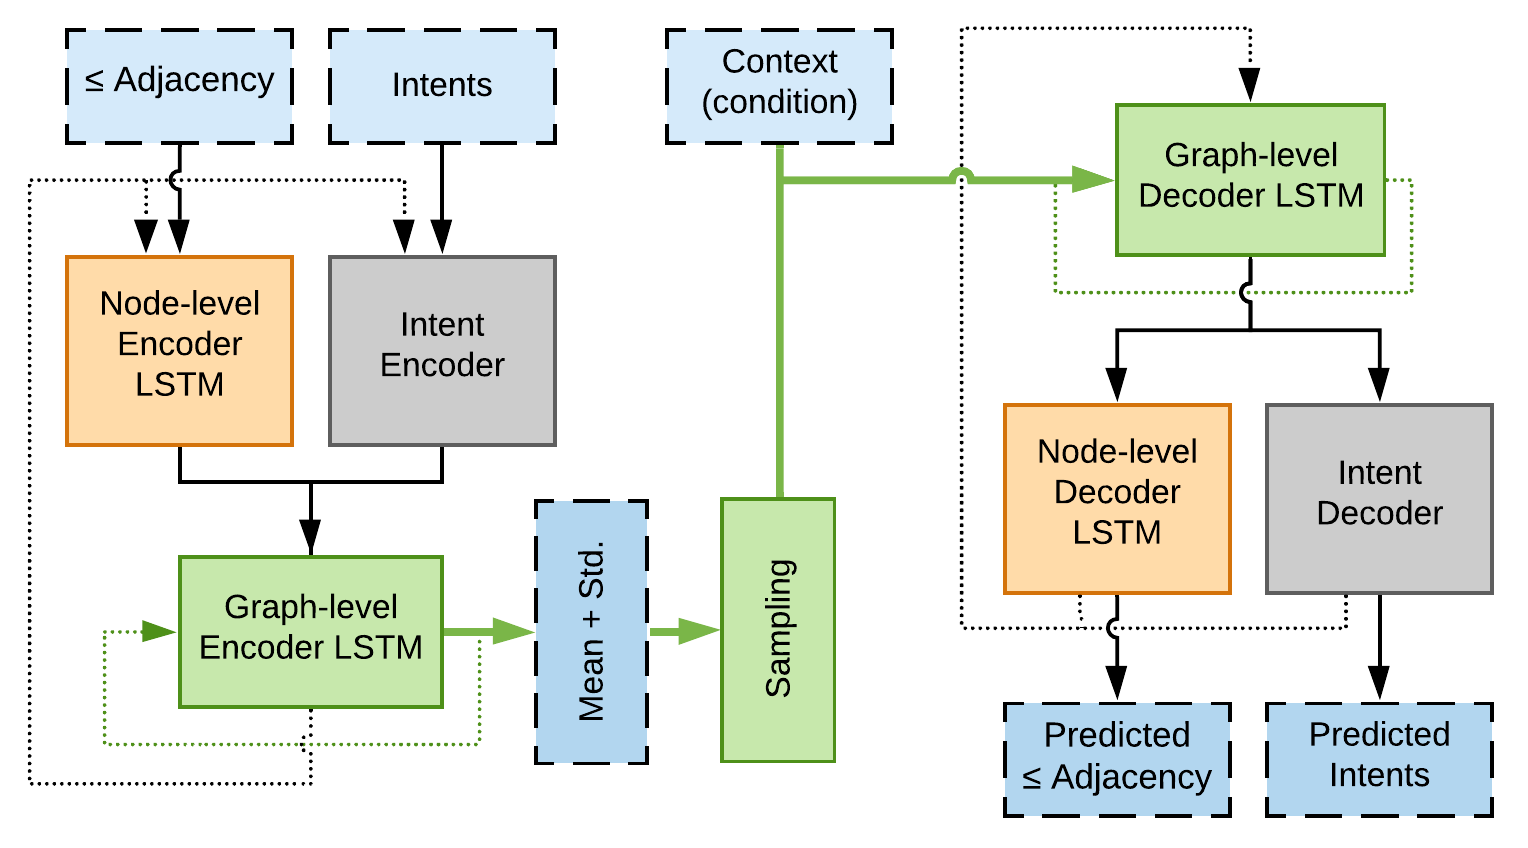
\includegraphics[keepaspectratio, width=.9\textwidth]{Figures/Ch1/grnn_full_.png}
    \caption{Adapted GraphRNN Constrained VAE.}
    \label{fig:graphrnn-cvae}
\end{figure}

The development plan is in 3 steps: \textit{(i)} building a VAE for lattices using the original GraphRNN design, \textit{(ii)} integrating the intent generation to the VAE, by extending the original GraphRNN design and \textit{(iii)} integrate the condition system.
The first two steps of the approach allow our model to first learn the representation of lattices in an auto-supervised manner, thanks to the auto-encoding principle.
At the issue of those two steps, the model should have learned ``what is a lattice''.
The third step is for developing the embedding of the FC.
This development process allows us to adapt the approach if one of the steps do not provide acceptable results.
Indeed, if the model does not manage to capture the basic structural properties of lattices (without the intents), it is unlikely that it will be able to handle the full complexity of the structure of lattices with the intents.
Similarly, if the model has trouble handling the full complexity of lattices, we won't be able to use it to generate lattices from FCs.


Our auto-encoder is composed of two GraphRNNs, one for the encoder and the other for the decoder.
The encoder GraphRNN reads the graph, and the last hidden state of the graph-level RNN is used to build the embedding.
The decoder GraphRNN is initialized with the embedding as the first hidden state of the graph-level RNN and generates.
To handle the concept intents, an intent model is added alongside the node-level model.
Similarly to the node-level, this second model takes the output of the graph-level model as its input.
Block diagrams of the folded encoder and decoder are shown in \cref{fig:graphrnn-autoencoder}.

%For the auto-encoder, we decided to share the parameters of the node-level RNN\todo{why?}

\begin{figure}
    \centering
    \subcaptionbox{Encoder\label{fig:graphrnn-encoder}}{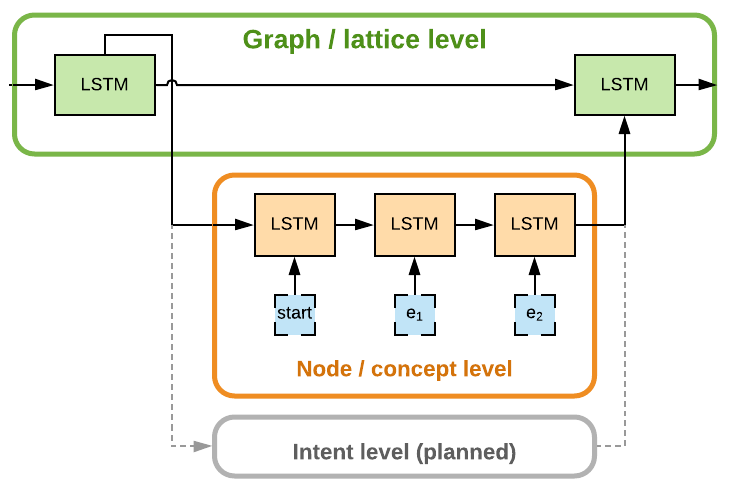
\includegraphics[keepaspectratio, width=.48\textwidth]{Figures/Ch1/grnn_encoder.png}}
    \subcaptionbox{Decoder\label{fig:graphrnn-decoder}}{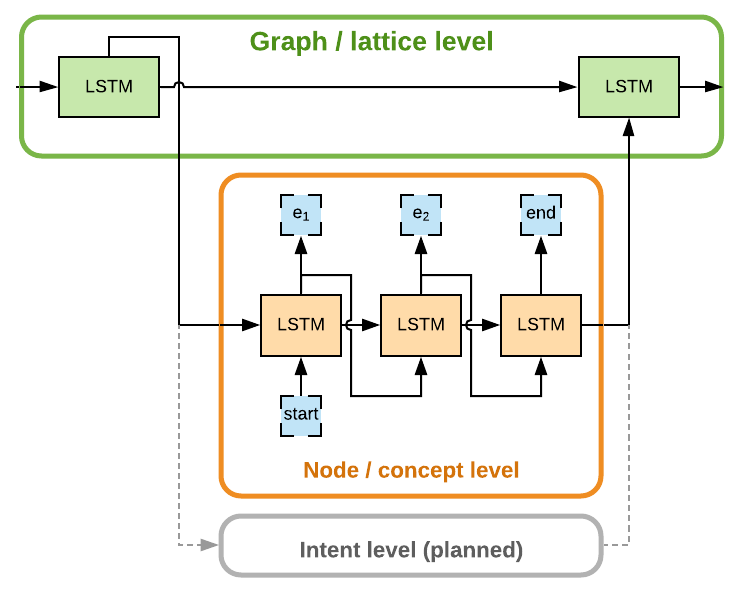
\includegraphics[keepaspectratio, width=.48\textwidth]{Figures/Ch1/grnn_decoder.png}}
    \caption{Details of the adapted GraphRNN, with edge and intent generation.}
    \label{fig:graphrnn-autoencoder}
\end{figure}